\section*{\nr.3 \titthree (10 Punkte)}
\begin{enumerate}[(a)]
\item Nach der erweiterten Kirchhoffschen Maschenregel gilt:
\begin{equation}
\hat{U}_e = R \hat{I} +\frac{1}{i\omega C}\hat{I} \iff \hat{I} =\frac{\hat{U}_e}{R+1/(iwC)}
\end{equation}

Setzen wir für die Eingangsspannung also $U_e=\hat{U}_e e^{i\omega t}$ an, ergibt sich der Strom durch $I=\hat{I} e^{i\omega t}$. Die Ausgangsspannung ist die Spannung über dem Kondensator, also:
\begin{equation}
U_a = \frac{1}{i\omega C}I = \frac{\hat{U}_e}{1+i\omega RC} e^{i\omega t}
\end{equation}
Für die Amplitude der Ausgangsspannung ergibt sich
\begin{equation}
|\hat{U}_a| = \hat{U}_e \left| \frac{1-i\omega RC}{1+(\omega R C)^2} \right| = \frac{\hat{U}_e}{\sqrt{1+(\omega R C)^2}},
\end{equation}
während für die Phasenverschiebung bei Betrachtung von Real- und Imaginärteil von $\hat{U}_a$ die Beziehung
\begin{equation}
\tan{\phi} = -\omega R C \iff \phi = -\arctan{\omega R C}
\end{equation}
gilt.
\item
Für das Verhältnis der Spannungsamplituden gilt mit $\omega_0 := 1/(RC)$:
\begin{equation}
\frac{\hat{U}_a}{\hat{U}_e} = \frac{1}{\sqrt{1+(\omega R C )^2}} = \frac{1}{\sqrt{1+(\omega/\omega_0)^2}}
\end{equation}
Für die Phasenverschiebung findet sich analog:
\begin{equation}
\phi = -\arctan (\omega/\omega_0)
\end{equation}
Abbildungen der funktionalen Zusammenhänge sind durch \vref{fig:tiefpassfig} gegeben.
\begin{figure}[htbp]
\centering
% GNUPLOT: LaTeX picture with Postscript
\begingroup
  \makeatletter
  \providecommand\color[2][]{%
    \GenericError{(gnuplot) \space\space\space\@spaces}{%
      Package color not loaded in conjunction with
      terminal option `colourtext'%
    }{See the gnuplot documentation for explanation.%
    }{Either use 'blacktext' in gnuplot or load the package
      color.sty in LaTeX.}%
    \renewcommand\color[2][]{}%
  }%
  \providecommand\includegraphics[2][]{%
    \GenericError{(gnuplot) \space\space\space\@spaces}{%
      Package graphicx or graphics not loaded%
    }{See the gnuplot documentation for explanation.%
    }{The gnuplot epslatex terminal needs graphicx.sty or graphics.sty.}%
    \renewcommand\includegraphics[2][]{}%
  }%
  \providecommand\rotatebox[2]{#2}%
  \@ifundefined{ifGPcolor}{%
    \newif\ifGPcolor
    \GPcolortrue
  }{}%
  \@ifundefined{ifGPblacktext}{%
    \newif\ifGPblacktext
    \GPblacktextfalse
  }{}%
  % define a \g@addto@macro without @ in the name:
  \let\gplgaddtomacro\g@addto@macro
  % define empty templates for all commands taking text:
  \gdef\gplbacktext{}%
  \gdef\gplfronttext{}%
  \makeatother
  \ifGPblacktext
    % no textcolor at all
    \def\colorrgb#1{}%
    \def\colorgray#1{}%
  \else
    % gray or color?
    \ifGPcolor
      \def\colorrgb#1{\color[rgb]{#1}}%
      \def\colorgray#1{\color[gray]{#1}}%
      \expandafter\def\csname LTw\endcsname{\color{white}}%
      \expandafter\def\csname LTb\endcsname{\color{black}}%
      \expandafter\def\csname LTa\endcsname{\color{black}}%
      \expandafter\def\csname LT0\endcsname{\color[rgb]{1,0,0}}%
      \expandafter\def\csname LT1\endcsname{\color[rgb]{0,1,0}}%
      \expandafter\def\csname LT2\endcsname{\color[rgb]{0,0,1}}%
      \expandafter\def\csname LT3\endcsname{\color[rgb]{1,0,1}}%
      \expandafter\def\csname LT4\endcsname{\color[rgb]{0,1,1}}%
      \expandafter\def\csname LT5\endcsname{\color[rgb]{1,1,0}}%
      \expandafter\def\csname LT6\endcsname{\color[rgb]{0,0,0}}%
      \expandafter\def\csname LT7\endcsname{\color[rgb]{1,0.3,0}}%
      \expandafter\def\csname LT8\endcsname{\color[rgb]{0.5,0.5,0.5}}%
    \else
      % gray
      \def\colorrgb#1{\color{black}}%
      \def\colorgray#1{\color[gray]{#1}}%
      \expandafter\def\csname LTw\endcsname{\color{white}}%
      \expandafter\def\csname LTb\endcsname{\color{black}}%
      \expandafter\def\csname LTa\endcsname{\color{black}}%
      \expandafter\def\csname LT0\endcsname{\color{black}}%
      \expandafter\def\csname LT1\endcsname{\color{black}}%
      \expandafter\def\csname LT2\endcsname{\color{black}}%
      \expandafter\def\csname LT3\endcsname{\color{black}}%
      \expandafter\def\csname LT4\endcsname{\color{black}}%
      \expandafter\def\csname LT5\endcsname{\color{black}}%
      \expandafter\def\csname LT6\endcsname{\color{black}}%
      \expandafter\def\csname LT7\endcsname{\color{black}}%
      \expandafter\def\csname LT8\endcsname{\color{black}}%
    \fi
  \fi
    \setlength{\unitlength}{0.0500bp}%
    \ifx\gptboxheight\undefined%
      \newlength{\gptboxheight}%
      \newlength{\gptboxwidth}%
      \newsavebox{\gptboxtext}%
    \fi%
    \setlength{\fboxrule}{0.5pt}%
    \setlength{\fboxsep}{1pt}%
\begin{picture}(4534.00,3400.00)%
    \gplgaddtomacro\gplbacktext{%
      \csname LTb\endcsname%
      \put(814,907){\makebox(0,0)[r]{\strut{}$0$}}%
      \put(814,1514){\makebox(0,0)[r]{\strut{}$0.3$}}%
      \put(814,2122){\makebox(0,0)[r]{\strut{}$0.6$}}%
      \put(814,2730){\makebox(0,0)[r]{\strut{}$0.9$}}%
      \put(1549,484){\makebox(0,0){\strut{}$0.1$}}%
      \put(2412,484){\makebox(0,0){\strut{}$1$}}%
      \put(3274,484){\makebox(0,0){\strut{}$10$}}%
      \put(4137,484){\makebox(0,0){\strut{}$100$}}%
    }%
    \gplgaddtomacro\gplfronttext{%
      \csname LTb\endcsname%
      \put(176,1919){\rotatebox{-270}{\makebox(0,0){\strut{}$\hat{U}_a/\hat{U}_e$}}}%
      \put(2541,154){\makebox(0,0){\strut{}$\omega/\omega_0$}}%
    }%
    \gplgaddtomacro\gplbacktext{%
      \csname LTb\endcsname%
      \put(814,907){\makebox(0,0)[r]{\strut{}$0$}}%
      \put(814,1514){\makebox(0,0)[r]{\strut{}$0.3$}}%
      \put(814,2122){\makebox(0,0)[r]{\strut{}$0.6$}}%
      \put(814,2730){\makebox(0,0)[r]{\strut{}$0.9$}}%
      \put(1549,484){\makebox(0,0){\strut{}$0.1$}}%
      \put(2412,484){\makebox(0,0){\strut{}$1$}}%
      \put(3274,484){\makebox(0,0){\strut{}$10$}}%
      \put(4137,484){\makebox(0,0){\strut{}$100$}}%
    }%
    \gplgaddtomacro\gplfronttext{%
      \csname LTb\endcsname%
      \put(176,1919){\rotatebox{-270}{\makebox(0,0){\strut{}$\hat{U}_a/\hat{U}_e$}}}%
      \put(2541,154){\makebox(0,0){\strut{}$\omega/\omega_0$}}%
    }%
    \gplbacktext
    \put(0,0){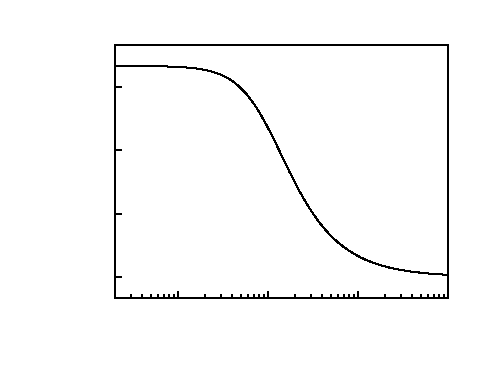
\includegraphics{output-plotU}}%
    \gplfronttext
  \end{picture}%
\endgroup
\hfill
% GNUPLOT: LaTeX picture with Postscript
\begingroup
  \makeatletter
  \providecommand\color[2][]{%
    \GenericError{(gnuplot) \space\space\space\@spaces}{%
      Package color not loaded in conjunction with
      terminal option `colourtext'%
    }{See the gnuplot documentation for explanation.%
    }{Either use 'blacktext' in gnuplot or load the package
      color.sty in LaTeX.}%
    \renewcommand\color[2][]{}%
  }%
  \providecommand\includegraphics[2][]{%
    \GenericError{(gnuplot) \space\space\space\@spaces}{%
      Package graphicx or graphics not loaded%
    }{See the gnuplot documentation for explanation.%
    }{The gnuplot epslatex terminal needs graphicx.sty or graphics.sty.}%
    \renewcommand\includegraphics[2][]{}%
  }%
  \providecommand\rotatebox[2]{#2}%
  \@ifundefined{ifGPcolor}{%
    \newif\ifGPcolor
    \GPcolortrue
  }{}%
  \@ifundefined{ifGPblacktext}{%
    \newif\ifGPblacktext
    \GPblacktextfalse
  }{}%
  % define a \g@addto@macro without @ in the name:
  \let\gplgaddtomacro\g@addto@macro
  % define empty templates for all commands taking text:
  \gdef\gplbacktext{}%
  \gdef\gplfronttext{}%
  \makeatother
  \ifGPblacktext
    % no textcolor at all
    \def\colorrgb#1{}%
    \def\colorgray#1{}%
  \else
    % gray or color?
    \ifGPcolor
      \def\colorrgb#1{\color[rgb]{#1}}%
      \def\colorgray#1{\color[gray]{#1}}%
      \expandafter\def\csname LTw\endcsname{\color{white}}%
      \expandafter\def\csname LTb\endcsname{\color{black}}%
      \expandafter\def\csname LTa\endcsname{\color{black}}%
      \expandafter\def\csname LT0\endcsname{\color[rgb]{1,0,0}}%
      \expandafter\def\csname LT1\endcsname{\color[rgb]{0,1,0}}%
      \expandafter\def\csname LT2\endcsname{\color[rgb]{0,0,1}}%
      \expandafter\def\csname LT3\endcsname{\color[rgb]{1,0,1}}%
      \expandafter\def\csname LT4\endcsname{\color[rgb]{0,1,1}}%
      \expandafter\def\csname LT5\endcsname{\color[rgb]{1,1,0}}%
      \expandafter\def\csname LT6\endcsname{\color[rgb]{0,0,0}}%
      \expandafter\def\csname LT7\endcsname{\color[rgb]{1,0.3,0}}%
      \expandafter\def\csname LT8\endcsname{\color[rgb]{0.5,0.5,0.5}}%
    \else
      % gray
      \def\colorrgb#1{\color{black}}%
      \def\colorgray#1{\color[gray]{#1}}%
      \expandafter\def\csname LTw\endcsname{\color{white}}%
      \expandafter\def\csname LTb\endcsname{\color{black}}%
      \expandafter\def\csname LTa\endcsname{\color{black}}%
      \expandafter\def\csname LT0\endcsname{\color{black}}%
      \expandafter\def\csname LT1\endcsname{\color{black}}%
      \expandafter\def\csname LT2\endcsname{\color{black}}%
      \expandafter\def\csname LT3\endcsname{\color{black}}%
      \expandafter\def\csname LT4\endcsname{\color{black}}%
      \expandafter\def\csname LT5\endcsname{\color{black}}%
      \expandafter\def\csname LT6\endcsname{\color{black}}%
      \expandafter\def\csname LT7\endcsname{\color{black}}%
      \expandafter\def\csname LT8\endcsname{\color{black}}%
    \fi
  \fi
    \setlength{\unitlength}{0.0500bp}%
    \ifx\gptboxheight\undefined%
      \newlength{\gptboxheight}%
      \newlength{\gptboxwidth}%
      \newsavebox{\gptboxtext}%
    \fi%
    \setlength{\fboxrule}{0.5pt}%
    \setlength{\fboxsep}{1pt}%
\begin{picture}(4534.00,3400.00)%
    \gplgaddtomacro\gplbacktext{%
      \csname LTb\endcsname%
      \put(946,839){\makebox(0,0)[r]{\strut{}$-1.6$}}%
      \put(946,1379){\makebox(0,0)[r]{\strut{}$-1.2$}}%
      \put(946,1919){\makebox(0,0)[r]{\strut{}$-0.8$}}%
      \put(946,2460){\makebox(0,0)[r]{\strut{}$-0.4$}}%
      \put(946,3000){\makebox(0,0)[r]{\strut{}$0$}}%
      \put(1656,484){\makebox(0,0){\strut{}$0.1$}}%
      \put(2483,484){\makebox(0,0){\strut{}$1$}}%
      \put(3310,484){\makebox(0,0){\strut{}$10$}}%
      \put(4137,484){\makebox(0,0){\strut{}$100$}}%
    }%
    \gplgaddtomacro\gplfronttext{%
      \csname LTb\endcsname%
      \put(176,1919){\rotatebox{-270}{\makebox(0,0){\strut{}$\phi$}}}%
      \put(2607,154){\makebox(0,0){\strut{}$\omega/\omega_0$}}%
    }%
    \gplgaddtomacro\gplbacktext{%
      \csname LTb\endcsname%
      \put(946,839){\makebox(0,0)[r]{\strut{}$-1.6$}}%
      \put(946,1379){\makebox(0,0)[r]{\strut{}$-1.2$}}%
      \put(946,1919){\makebox(0,0)[r]{\strut{}$-0.8$}}%
      \put(946,2460){\makebox(0,0)[r]{\strut{}$-0.4$}}%
      \put(946,3000){\makebox(0,0)[r]{\strut{}$0$}}%
      \put(1656,484){\makebox(0,0){\strut{}$0.1$}}%
      \put(2483,484){\makebox(0,0){\strut{}$1$}}%
      \put(3310,484){\makebox(0,0){\strut{}$10$}}%
      \put(4137,484){\makebox(0,0){\strut{}$100$}}%
    }%
    \gplgaddtomacro\gplfronttext{%
      \csname LTb\endcsname%
      \put(176,1919){\rotatebox{-270}{\makebox(0,0){\strut{}$\phi$}}}%
      \put(2607,154){\makebox(0,0){\strut{}$\omega/\omega_0$}}%
    }%
    \gplbacktext
    \put(0,0){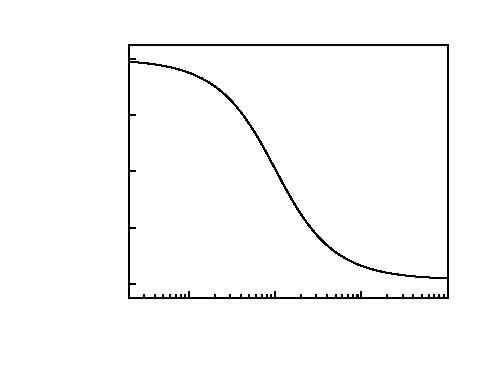
\includegraphics{output-plotphi}}%
    \gplfronttext
  \end{picture}%
\endgroup

\caption{Links das Verhältnis $\hat{U}_a/\hat{U}_e$, rechts die Phasenverschiebung, jeweils in logarithmischer Skalierung der $x$-Achse.}
\label{fig:tiefpassfig}
\end{figure}

\item Bei kleinen Frequenzen kann sich der Kondensator teilweise aufladen, wodurch sich eine Potentialdifferenz am Ausgang aufbaut. Das Verhältnis aus Ausgangs- und Eingangsspannung ist dadurch hoch. Bei höheren Frequenzen wirkt der Kondensator als bloßes Kabel, wodurch das obige Verhältnis sinkt.

Betrachtet man den Graphen der Phasenverschiebung, so ist sie negativ. Die Ausgangsspannung eilt also der Eingangsspannung voraus, und zwar umso weiter, je höher die Frequenz ist. 

\end{enumerate}